\documentclass[]{article}
\usepackage{lmodern}
\usepackage{amssymb,amsmath}
\usepackage{ifxetex,ifluatex}
\usepackage{fixltx2e} % provides \textsubscript
\ifnum 0\ifxetex 1\fi\ifluatex 1\fi=0 % if pdftex
  \usepackage[T1]{fontenc}
  \usepackage[utf8]{inputenc}
\else % if luatex or xelatex
  \ifxetex
    \usepackage{mathspec}
  \else
    \usepackage{fontspec}
  \fi
  \defaultfontfeatures{Ligatures=TeX,Scale=MatchLowercase}
\fi
% use upquote if available, for straight quotes in verbatim environments
\IfFileExists{upquote.sty}{\usepackage{upquote}}{}
% use microtype if available
\IfFileExists{microtype.sty}{%
\usepackage{microtype}
\UseMicrotypeSet[protrusion]{basicmath} % disable protrusion for tt fonts
}{}
\usepackage[margin=1in]{geometry}
\usepackage{hyperref}
\hypersetup{unicode=true,
            pdftitle={Ant on a stick},
            pdfauthor={Chao XIA},
            pdfborder={0 0 0},
            breaklinks=true}
\urlstyle{same}  % don't use monospace font for urls
\usepackage{color}
\usepackage{fancyvrb}
\newcommand{\VerbBar}{|}
\newcommand{\VERB}{\Verb[commandchars=\\\{\}]}
\DefineVerbatimEnvironment{Highlighting}{Verbatim}{commandchars=\\\{\}}
% Add ',fontsize=\small' for more characters per line
\usepackage{framed}
\definecolor{shadecolor}{RGB}{248,248,248}
\newenvironment{Shaded}{\begin{snugshade}}{\end{snugshade}}
\newcommand{\KeywordTok}[1]{\textcolor[rgb]{0.13,0.29,0.53}{\textbf{#1}}}
\newcommand{\DataTypeTok}[1]{\textcolor[rgb]{0.13,0.29,0.53}{#1}}
\newcommand{\DecValTok}[1]{\textcolor[rgb]{0.00,0.00,0.81}{#1}}
\newcommand{\BaseNTok}[1]{\textcolor[rgb]{0.00,0.00,0.81}{#1}}
\newcommand{\FloatTok}[1]{\textcolor[rgb]{0.00,0.00,0.81}{#1}}
\newcommand{\ConstantTok}[1]{\textcolor[rgb]{0.00,0.00,0.00}{#1}}
\newcommand{\CharTok}[1]{\textcolor[rgb]{0.31,0.60,0.02}{#1}}
\newcommand{\SpecialCharTok}[1]{\textcolor[rgb]{0.00,0.00,0.00}{#1}}
\newcommand{\StringTok}[1]{\textcolor[rgb]{0.31,0.60,0.02}{#1}}
\newcommand{\VerbatimStringTok}[1]{\textcolor[rgb]{0.31,0.60,0.02}{#1}}
\newcommand{\SpecialStringTok}[1]{\textcolor[rgb]{0.31,0.60,0.02}{#1}}
\newcommand{\ImportTok}[1]{#1}
\newcommand{\CommentTok}[1]{\textcolor[rgb]{0.56,0.35,0.01}{\textit{#1}}}
\newcommand{\DocumentationTok}[1]{\textcolor[rgb]{0.56,0.35,0.01}{\textbf{\textit{#1}}}}
\newcommand{\AnnotationTok}[1]{\textcolor[rgb]{0.56,0.35,0.01}{\textbf{\textit{#1}}}}
\newcommand{\CommentVarTok}[1]{\textcolor[rgb]{0.56,0.35,0.01}{\textbf{\textit{#1}}}}
\newcommand{\OtherTok}[1]{\textcolor[rgb]{0.56,0.35,0.01}{#1}}
\newcommand{\FunctionTok}[1]{\textcolor[rgb]{0.00,0.00,0.00}{#1}}
\newcommand{\VariableTok}[1]{\textcolor[rgb]{0.00,0.00,0.00}{#1}}
\newcommand{\ControlFlowTok}[1]{\textcolor[rgb]{0.13,0.29,0.53}{\textbf{#1}}}
\newcommand{\OperatorTok}[1]{\textcolor[rgb]{0.81,0.36,0.00}{\textbf{#1}}}
\newcommand{\BuiltInTok}[1]{#1}
\newcommand{\ExtensionTok}[1]{#1}
\newcommand{\PreprocessorTok}[1]{\textcolor[rgb]{0.56,0.35,0.01}{\textit{#1}}}
\newcommand{\AttributeTok}[1]{\textcolor[rgb]{0.77,0.63,0.00}{#1}}
\newcommand{\RegionMarkerTok}[1]{#1}
\newcommand{\InformationTok}[1]{\textcolor[rgb]{0.56,0.35,0.01}{\textbf{\textit{#1}}}}
\newcommand{\WarningTok}[1]{\textcolor[rgb]{0.56,0.35,0.01}{\textbf{\textit{#1}}}}
\newcommand{\AlertTok}[1]{\textcolor[rgb]{0.94,0.16,0.16}{#1}}
\newcommand{\ErrorTok}[1]{\textcolor[rgb]{0.64,0.00,0.00}{\textbf{#1}}}
\newcommand{\NormalTok}[1]{#1}
\usepackage{graphicx,grffile}
\makeatletter
\def\maxwidth{\ifdim\Gin@nat@width>\linewidth\linewidth\else\Gin@nat@width\fi}
\def\maxheight{\ifdim\Gin@nat@height>\textheight\textheight\else\Gin@nat@height\fi}
\makeatother
% Scale images if necessary, so that they will not overflow the page
% margins by default, and it is still possible to overwrite the defaults
% using explicit options in \includegraphics[width, height, ...]{}
\setkeys{Gin}{width=\maxwidth,height=\maxheight,keepaspectratio}
\IfFileExists{parskip.sty}{%
\usepackage{parskip}
}{% else
\setlength{\parindent}{0pt}
\setlength{\parskip}{6pt plus 2pt minus 1pt}
}
\setlength{\emergencystretch}{3em}  % prevent overfull lines
\providecommand{\tightlist}{%
  \setlength{\itemsep}{0pt}\setlength{\parskip}{0pt}}
\setcounter{secnumdepth}{0}
% Redefines (sub)paragraphs to behave more like sections
\ifx\paragraph\undefined\else
\let\oldparagraph\paragraph
\renewcommand{\paragraph}[1]{\oldparagraph{#1}\mbox{}}
\fi
\ifx\subparagraph\undefined\else
\let\oldsubparagraph\subparagraph
\renewcommand{\subparagraph}[1]{\oldsubparagraph{#1}\mbox{}}
\fi

%%% Use protect on footnotes to avoid problems with footnotes in titles
\let\rmarkdownfootnote\footnote%
\def\footnote{\protect\rmarkdownfootnote}

%%% Change title format to be more compact
\usepackage{titling}

% Create subtitle command for use in maketitle
\newcommand{\subtitle}[1]{
  \posttitle{
    \begin{center}\large#1\end{center}
    }
}

\setlength{\droptitle}{-2em}

  \title{Ant on a stick}
    \pretitle{\vspace{\droptitle}\centering\huge}
  \posttitle{\par}
    \author{Chao XIA}
    \preauthor{\centering\large\emph}
  \postauthor{\par}
      \predate{\centering\large\emph}
  \postdate{\par}
    \date{01/23/2019}

\usepackage{ctex}

\begin{document}
\maketitle

\subsection{Introduction}\label{introduction}

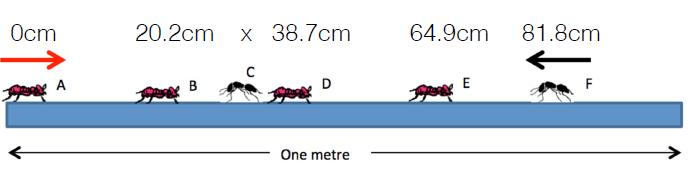
\includegraphics{ant.jpg}\\
Ants walk at 1cm/second. When they meet, each ant turns around and walks
in the other direction. When they reach the end of the stick they fall
off.

\begin{enumerate}
\def\labelenumi{(\arabic{enumi})}
\item
  How many seconds until the last ant falls off?
\item
  Which ant is the last to fall off the stick?
\end{enumerate}

\subsection{Solution}\label{solution}

Creat three vector:

\begin{enumerate}
\def\labelenumi{(\arabic{enumi})}
\item
  Flag: represent the label of each ant;
\item
  Speed: represent the speed of each ant in the flag vector;
\item
  Location: represent the location of each ant in the flag vector from
  the 0 point on the stick;
\end{enumerate}

Examine the location of each ant each second. Since ants which go to
left only meet the ant on the left of it, when the location of ants
which goes to left is smaller than that of the ant on the left of it,
their location and speed will be changed.

Here is the code:

\begin{Shaded}
\begin{Highlighting}[]
\KeywordTok{set.seed}\NormalTok{(}\DecValTok{789}\NormalTok{)}
\NormalTok{Time <-}\StringTok{ }\KeywordTok{numeric}\NormalTok{()}
\NormalTok{Last <-}\StringTok{ }\KeywordTok{vector}\NormalTok{()}
\NormalTok{ant <-}\StringTok{ }\ControlFlowTok{function}\NormalTok{(n)\{}
  \ControlFlowTok{for}\NormalTok{ (l }\ControlFlowTok{in} \DecValTok{1}\OperatorTok{:}\NormalTok{n)\{}
\NormalTok{    location <-}\StringTok{ }\KeywordTok{c}\NormalTok{(}\DecValTok{0}\NormalTok{, }\FloatTok{20.2}\NormalTok{, }\KeywordTok{runif}\NormalTok{(}\DecValTok{1}\NormalTok{,}\FloatTok{20.2}\NormalTok{,}\FloatTok{38.7}\NormalTok{), }\FloatTok{38.7}\NormalTok{, }\FloatTok{64.9}\NormalTok{, }\FloatTok{81.8}\NormalTok{) }\CommentTok{#define location of each ant}
\NormalTok{    flag <-}\StringTok{ }\KeywordTok{c}\NormalTok{(}\StringTok{'a'}\NormalTok{,}\StringTok{'b'}\NormalTok{,}\StringTok{'c'}\NormalTok{,}\StringTok{'d'}\NormalTok{,}\StringTok{'e'}\NormalTok{,}\StringTok{'f'}\NormalTok{) }\CommentTok{#define label of each ant}
\NormalTok{    speed <-}\StringTok{ }\KeywordTok{c}\NormalTok{(}\DecValTok{1}\NormalTok{,}\DecValTok{1}\NormalTok{,}\OperatorTok{-}\DecValTok{1}\NormalTok{,}\DecValTok{1}\NormalTok{,}\DecValTok{1}\NormalTok{,}\OperatorTok{-}\DecValTok{1}\NormalTok{) }\CommentTok{#define initial speed of eahc ant}
\NormalTok{    T <-}\StringTok{ }\DecValTok{0}
    \ControlFlowTok{while}\NormalTok{(}\KeywordTok{length}\NormalTok{(location)}\OperatorTok{>}\DecValTok{1}\NormalTok{)\{ }\CommentTok{# Examine if there is only one ant on the stick}
\NormalTok{      T <-}\StringTok{ }\NormalTok{T}\OperatorTok{+}\DecValTok{1} \CommentTok{# Time flows one second}
      \CommentTok{# The location of each ant changes}
      \ControlFlowTok{for}\NormalTok{ (i }\ControlFlowTok{in} \DecValTok{1}\OperatorTok{:}\KeywordTok{length}\NormalTok{(location))\{}
\NormalTok{        location[i] <-}\StringTok{ }\NormalTok{location[i] }\OperatorTok{+}\StringTok{ }\NormalTok{speed[i]}
\NormalTok{      \}}
      
\NormalTok{      left <-}\StringTok{ }\KeywordTok{which}\NormalTok{(speed }\OperatorTok{<}\StringTok{ }\DecValTok{0}\NormalTok{) }\CommentTok{# Find the ants go to left side}
      \CommentTok{# If the ant is not the most left side ant, compare its location with the ant on the left }
      \CommentTok{# of it. And if its location is lower the ant on the left of it, change their speed and location.}
      \ControlFlowTok{if}\NormalTok{(left[}\DecValTok{1}\NormalTok{] }\OperatorTok{>}\StringTok{ }\DecValTok{1}\NormalTok{)\{}
        \ControlFlowTok{for}\NormalTok{ (j }\ControlFlowTok{in} \DecValTok{1}\OperatorTok{:}\KeywordTok{length}\NormalTok{(left))\{}
          \ControlFlowTok{if}\NormalTok{ (location[left[j]] }\OperatorTok{<}\StringTok{ }\NormalTok{location[left[j]}\OperatorTok{-}\DecValTok{1}\NormalTok{])\{}
\NormalTok{            tmp1 <-}\StringTok{ }\NormalTok{speed[left[j]]  }
\NormalTok{            speed[left[j]] <-}\StringTok{ }\NormalTok{speed[left[j]}\OperatorTok{-}\DecValTok{1}\NormalTok{]}
\NormalTok{            speed[left[j]}\OperatorTok{-}\DecValTok{1}\NormalTok{] <-}\StringTok{ }\NormalTok{tmp1}
\NormalTok{            tmp2 <-}\StringTok{ }\NormalTok{location[left[j]]  }
\NormalTok{            location[left[j]] <-}\StringTok{ }\NormalTok{location[left[j]}\OperatorTok{-}\DecValTok{1}\NormalTok{]}
\NormalTok{            location[left[j]}\OperatorTok{-}\DecValTok{1}\NormalTok{] <-}\StringTok{ }\NormalTok{tmp2}
\NormalTok{          \}}
\NormalTok{        \}}
\NormalTok{      \} }
      \CommentTok{# Examine if there's ant fall off from the stick. If there is one, remove its label, location and speed.}
\NormalTok{      k <-}\StringTok{ }\DecValTok{1}
      \ControlFlowTok{while}\NormalTok{ (k }\OperatorTok{<=}\StringTok{ }\KeywordTok{length}\NormalTok{(location))\{}
        \ControlFlowTok{if}\NormalTok{ ((speed[k] }\OperatorTok{<}\StringTok{ }\DecValTok{0} \OperatorTok{&}\StringTok{ }\NormalTok{location[k] }\OperatorTok{<}\StringTok{ }\DecValTok{0}\NormalTok{) }\OperatorTok{|}\StringTok{ }\NormalTok{(speed[k] }\OperatorTok{>}\StringTok{ }\DecValTok{0} \OperatorTok{&}\StringTok{ }\NormalTok{location[k] }\OperatorTok{>}\StringTok{ }\DecValTok{100}\NormalTok{))\{}
\NormalTok{          location <-}\StringTok{ }\NormalTok{location[}\OperatorTok{-}\NormalTok{k]}
\NormalTok{          flag <-}\StringTok{ }\NormalTok{flag[}\OperatorTok{-}\NormalTok{k]}
\NormalTok{          speed <-}\StringTok{ }\NormalTok{speed[}\OperatorTok{-}\NormalTok{k]}
\NormalTok{        \}}
        \ControlFlowTok{else}\NormalTok{\{}
\NormalTok{        k <-}\StringTok{ }\NormalTok{k}\OperatorTok{+}\DecValTok{1}
\NormalTok{        \}}
\NormalTok{      \}}
\NormalTok{    \}}
\NormalTok{  T <-}\StringTok{ }\NormalTok{T }\OperatorTok{+}\StringTok{ }\DecValTok{100} \OperatorTok{-}\StringTok{ }\NormalTok{location }\CommentTok{#Total time equals to the sum of time flowed from the very beginning and the time the last ant on }
                          \CommentTok{#the stick will use to fall off from the stick}
\NormalTok{  Time[l] <-}\StringTok{ }\NormalTok{T}
\NormalTok{  Last[l] <-}\StringTok{ }\NormalTok{flag}
\NormalTok{  \}}
  \KeywordTok{cat}\NormalTok{(}\StringTok{'}\CharTok{\textbackslash{}n}\StringTok{It will be'}\NormalTok{, }\KeywordTok{mean}\NormalTok{(Time) ,}\StringTok{'seconds until last ant falls off.'}\NormalTok{)}
  \KeywordTok{cat}\NormalTok{(}\StringTok{'}\CharTok{\textbackslash{}n}\StringTok{Fot the last trial,'}\NormalTok{,flag,}\StringTok{'is the last ant to fall off.'}\NormalTok{)}
  \KeywordTok{as.data.frame}\NormalTok{(}\KeywordTok{table}\NormalTok{(Last))}
\NormalTok{\}}
\KeywordTok{ant}\NormalTok{(}\DecValTok{1}\NormalTok{)}
\end{Highlighting}
\end{Shaded}

\begin{verbatim}
## 
## It will be 100 seconds until last ant falls off.
## Fot the last trial, c is the last ant to fall off.
\end{verbatim}

\begin{verbatim}
##   Last Freq
## 1    c    1
\end{verbatim}

If we repeat the situation for 100 times.

\begin{Shaded}
\begin{Highlighting}[]
\KeywordTok{ant}\NormalTok{(}\DecValTok{100}\NormalTok{)}
\end{Highlighting}
\end{Shaded}

\begin{verbatim}
## 
## It will be 100 seconds until last ant falls off.
## Fot the last trial, c is the last ant to fall off.
\end{verbatim}

\begin{verbatim}
##   Last Freq
## 1    c  100
\end{verbatim}

In such case, we can know that it will be always 100 seconds until last
ant falls off from the stick and the last ant will always be No.C.


\end{document}
